% !TEX root = ../main.tex

\section{Methods}
\label{sec:data}

\subsection{Simulated data}

\begin{figure}[t!]
    \begin{center}
        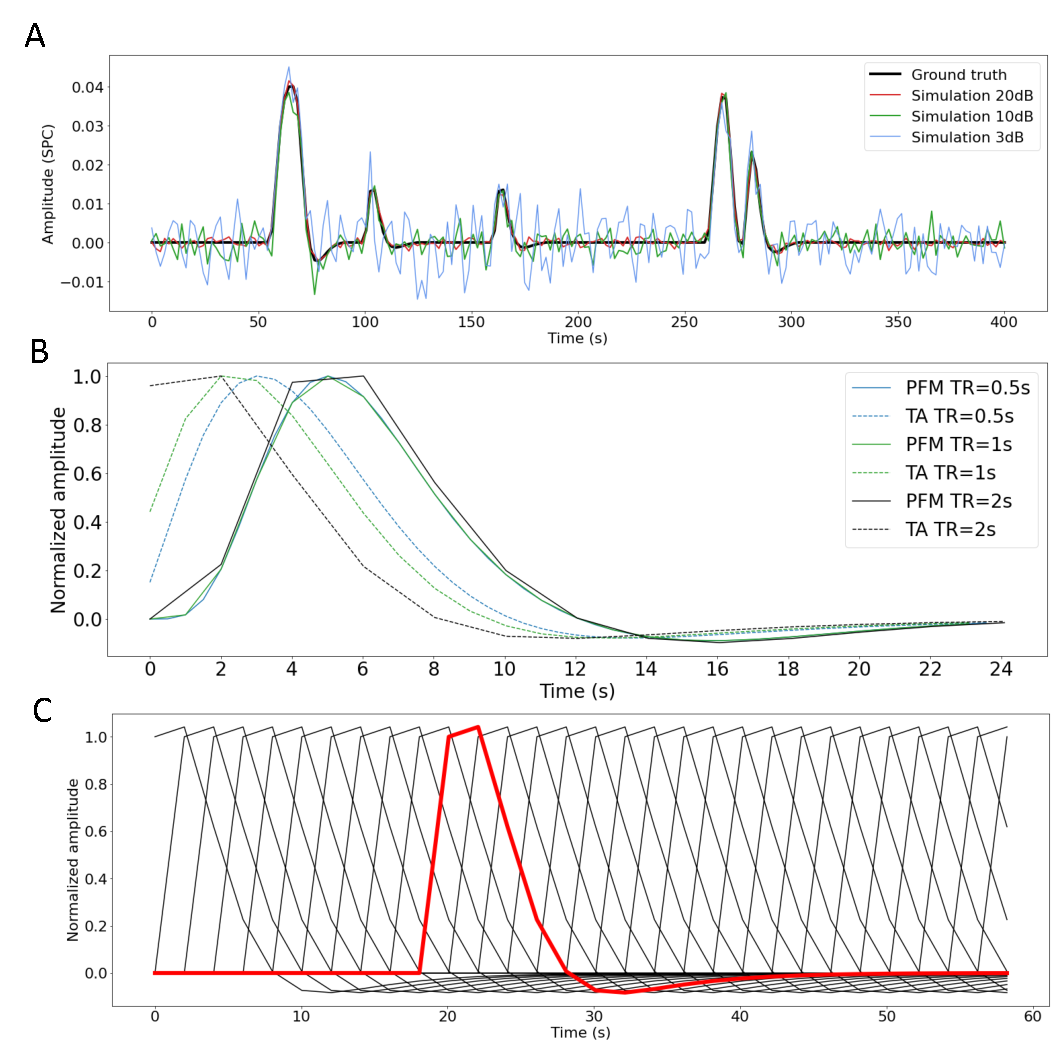
\includegraphics[width=0.75\columnwidth]{figures/sim_and_hrf.pdf}
    \end{center}
    \caption{A) Simulated signal with different SNRs (20 dB, 10 dB and 3 dB) and ground truth given in signal percentage change (SPC). B) Canonical HRF models typically used by PFM (solid line) and TA (dashed line) at TR = 0.5 s (blue), TR = 1 s (green) and TR = 2 s (black). Without loss of generality, the waveforms are scaled to unit amplitude for visualization. C) Representation of shifted HRFs at TR = 2 s that build the design matrix for PFM when the HRF model has been matched to that in TA. The red line corresponds to one of the columns of the HRF matrix.}
\label{fig:sim_and_hrf}
\end{figure}

In order to compare the two methods while controlling for their correct performance, we created a simulation scenario that can be found in the GitHub repository shared in Section~\ref{sec:github}. For the sake of illustration, we describe here the simulations corresponding to a timecourse with a duration of 400 seconds (TR = 2 s) where the activity-inducing signal includes 5 events, which are convolved with the canonical HRF. Different noise sources (physiological, thermal, and motion-related) were also added and we simulated three different scenarios with varying signal-to-noise ratios (SNR = [20 dB, 10 dB, 3 dB]) that represent high, medium and low contrast-to-noise ratios as shown in Figure~\ref{fig:sim_and_hrf}A. Noise was created following the procedure in (\citealt{Gaudes2013Paradigmfreemapping}) as the sum of uncorrelated Gaussian noise and sinusoidal signals to simulate a realistic noise model with thermal noise, cardiac and respiratory physiological fluctuations, respectively. The physiological signals were generated as
\begin{equation}
    \sum_{i=1}^{2} \frac{1}{2^{i-1}}\left(\sin \left(2 \pi f_{r, i} t+\phi_{\mathrm{r}, i}\right)+\sin \left(2 \pi f_{c, i} t+\phi_{c, i}\right)\right),
\end{equation}
with up to second-order harmonics per cardiac (\(f_{c,i}\)) and respiratory (\(f_{r,i}\)) component that were randomly generated following normal distributions with variance 0.04 and mean \(if_r\) and \(if_c\), for \(i = [1, 2]\). We set the fundamental frequencies to \(f_r = 0.3\) Hz for the respiratory component (\citealt{Birn2006Separatingrespiratoryvariation}) and \(f_c = 1.1\) Hz for the cardiac component (\citealt{Shmueli2007Lowfrequencyfluctuations}). The phases of each harmonic \(\phi\) were randomly selected from a uniform distribution between 0 and 2$\pi$ radians. To simulate physiological noise that is proportional to the change in BOLD signal, a variable ratio between the physiological (\(\sigma_P\)) and the thermal (\(\sigma_0\)) noise was modeled as \(\sigma_P/\sigma_0 = a(tSNR)^b + c\), where \(a = 5.01 \times 10^{-6}\), \(b = 2.81\), and \(c = 0.397\), following the experimental measures available in Table 3 from (\citealt{Triantafyllou2005Comparisonphysiologicalnoise}).

%%%%%%%%%%%%%%%%%%%%%%%%%%%%%%%%%%%%%%%%%%%%%%%%%%%%%%%%%%%
%%%%%%%%%%%%%%%%%%%%%%%%%%%%%%%%%%%%%%%%%%%%%%%%%%%%%%%%%%%
%%%%%%%%%%%%%%%%%%%%%%%%%%%%%%%%%%%%%%%%%%%%%%%%%%%%%%%%%%%
\subsection{Experimental data}
To compare the performance of the two approaches as well as illustrate their operation, we employ two representative experimental datasets.

\textbf{Motor task dataset:} One healthy subject was scanned in a 3T MR scanner (Siemens) under a Basque Center on Cognition, Brain and Language Review Board-approved protocol. T2*-weighted multi-echo fMRI data was acquired with a simultaneous-multislice multi-echo gradient echo-planar imaging sequence, kindly provided by the Center of Magnetic Resonance Research (University of Minnesota, USA) (\citealt{Feinberg_2010,Moeller_2010,Setsompop_2011}), with the following parameters: 340 scans, 52 slices, Partial-Fourier = 6/8, voxel size = $2.4\times2.4\times3$ mm\textsuperscript{3}, TR = 1.5 s, TEs = 10.6/28.69/46.78/64.87/82.96 ms, flip angle = 70\(^o\), multiband factor = 4, GRAPPA = 2.

During the fMRI acquisition, the subject performed a motor task consisting of five different movements (left-hand finger tapping, right-hand finger tapping, moving the left toes, moving the right toes and moving the tongue) that were visually cued through a mirror located on the head coil. These conditions were randomly intermixed every 16 seconds, and were only repeated once the entire set of stimuli were presented. Data preprocessing consisted of first, discarding the first 10 volumes of the functional data to achieve a steady state of magnetization. Then, image realignment to the skull-stripped single-band reference image (SBRef) was computed on the first echo, and the estimated rigid-body spatial transformation was applied to all other echoes (\citealt{Jenkinson2012FSL,Jenkinson_2001}). A brain mask obtained from the SBRef volume was applied to all the echoes and the different echo timeseries were optimally combined (OC) voxelwise by weighting each timeseries contribution by its T2* value (\citealt{Posse_1999}). AFNI (\citealt{Cox1996AFNISoftwareAnalysis}) was employed for a detrending of up to 4\textsuperscript{th}-order Legendre polynomials, within-brain spatial smoothing (3 mm FWHM) and voxelwise signal normalization to percentage change. Finally, distortion field correction was performed on the OC volume with Topup (\citealt{Andersson_2003}), using the pair of spin-echo EPI images with reversed phase encoding acquired before the ME-EPI acquisition (\citealt{Glasser_2016}).

\textbf{Resting-state datasets:} One healthy subject was scanned in a 3T MR scanner (Siemens) under a Basque Center on Cognition, Brain and Language Review Board-approved protocol. Two runs of T2*-weighted fMRI data were acquired during resting-state, each with 10 min duration, with 1) a standard gradient-echo echo-planar imaging sequence (monoband) (TR = 2000 ms, TE = 29 ms, flip-angle = 78\(^o\), matrix size = $64\times64$, voxel size = $3\times3\times3$ mm\textsuperscript{3}, 33 axial slices with interleaved acquisition, slice gap = 0.6 mm) and 2) a  simultaneous-multislice gradient-echo echo-planar imaging sequence (multiband factor = 3, TR = 800 ms, TE = 29 ms, flip-angle = 60\(^o\), matrix size = $64\times64$, voxel size = $3\times3\times3$ mm\textsuperscript{3}, 42 axial slices with interleaved acquisition, no slice gap). Single-band reference images were also collected in both resting-state acquisitions for head motion realignment. Field maps were also obtained to correct for field distortions.

During both acquisitions, participants were instructed to keep their eyes open, fixating a white cross that they saw through a mirror located on the head coil, and not to think about anything specific. The data was pre-processed using AFNI (\citealt{Cox1996AFNISoftwareAnalysis}). First, volumes corresponding to the initial 10 seconds were removed to allow for a steady-state magnetization. Then, the voxel time-series were despiked to reduce large-amplitude deviations and slice-time corrected. Inhomogeneities caused by magnetic susceptibility were corrected with FUGUE (FSL) using the field map images (\citealt{Jenkinson2012FSL}). Next, functional images were realigned to a base volume (monoband: volume with the lowest head motion; multiband: single-band reference image). Finally, a simultaneous nuisance regression step was performed comprising up to 6\textsuperscript{th}-order Legendre polynomials, low-pass filtering with a cutoff frequency of 0.25 Hz (only on multiband data to match the frequency content of the monoband), 6 realignment parameters plus temporal derivatives, 5 principal components of white matter (WM), 5 principal components of lateral ventricle voxels (anatomical CompCor) (\citealt{Behzadi_2007}) and 5 principal components of the brain's edge voxels ,(\citealt{Patriat_2015}). WM, CSF and brain's edge-voxel masks were obtained from Freesurfer tissue and brain segmentations. In addition, scans with potential artifacts were identified and censored when the euclidean norm of the temporal derivative of the realignment parameters (ENORM) was larger than 0.4, and the proportion of voxels adjusted in the despiking step exceeded 10\%.

%%%%%%%%%%%%%%%%%%%%%%%%%%%%%%%%%%%%%%%%%%%%%%%%%%%%%%%%%%%
%%%%%%%%%%%%%%%%%%%%%%%%%%%%%%%%%%%%%%%%%%%%%%%%%%%%%%%%%%%
%%%%%%%%%%%%%%%%%%%%%%%%%%%%%%%%%%%%%%%%%%%%%%%%%%%%%%%%%%%
\subsection{Selection of the hemodynamic response function}

In their original formulations, PFM and TA specify the discrete-time HRF in different ways. For PFM, the continuous-domain specification of the canonical double-gamma HRF (\citealt{HENSON2007178}) is sampled at the TR and then put as shifted impulse responses to build the matrix $\mathbf{H}$.  In the case of TA, however, the continuous-domain linearized version of the balloon-windkessel model is discretized to build the linear differential operator in $\mathbf{D_H}$. While the TR only changes the resolution of the HRF shape for PFM, the impact of an equivalent impulse response of the discretized differential operator at different TR is more pronounced. As shown in Figure~\ref{fig:sim_and_hrf}B, longer TR leads to equivalent impulse responses of TA that are shifted in time, provoking a lack of the initial baseline and rise of the response. We refer the reader to Figure {\ref{fig:hrf_differences}} to see the differences in the estimation of the activity-inducing and innovation signals when both methods use the HRF in their original formulation. To avoid differences between PFM and TA based on their built-in HRF, we choose to build the synthesis operator $\mathbf{H}$ with shifted versions of the HRF given by the TA analysis operator (e.g., see Figure~\ref{fig:sim_and_hrf}C for the TR=2s case).

%%%%%%%%%%%%%%%%%%%%%%%%%%%%%%%%%%%%%%%%%%%%%%%%%%%%%%%%%%%
%%%%%%%%%%%%%%%%%%%%%%%%%%%%%%%%%%%%%%%%%%%%%%%%%%%%%%%%%%%
%%%%%%%%%%%%%%%%%%%%%%%%%%%%%%%%%%%%%%%%%%%%%%%%%%%%%%%%%%%
\subsection{Selection of the regularization parameter}

We use the simulated data to compare the performance of the two deconvolution algorithms with both BIC and MAD criteria to set the regularization parameter $\lambda$ (see section \ref{sec:regparam}). We also evaluate if the algorithms behave differently in terms of the estimation of the activity-inducing signal $\mathbf{\hat{s}}$ using the spike model described in~\eqref{eq:pfm_spike} and the block model based on the innovation signal $\mathbf{\hat{u}}$ in~\eqref{eq:pfm_block}.

For selection based on the BIC, LARS was initally performed with the PFM deconvolution model to obtain the solution for every possible $\lambda$ in the regularization path. Then, the values of $\lambda$ corresponding to the BIC optimum were adopted to solve the TA deconvolution model by means of FISTA. 

For a selection based on the MAD estimate of the noise, we apply the temporal regularization in its original form for TA, whereas for PFM the selected $\lambda$ corresponds to the solution whose residuals have the closest standard deviation to the estimated noise level of the data $\hat{\sigma}$.  %We do not introduce additional spatial regularization in any of the cases.

%%%%%%%%%%%%%%%%%%%%%%%%%%%%%%%%%%%%%%%%%%%%%%%%%%%%%%%%%%%
%%%%%%%%%%%%%%%%%%%%%%%%%%%%%%%%%%%%%%%%%%%%%%%%%%%%%%%%%%%
%%%%%%%%%%%%%%%%%%%%%%%%%%%%%%%%%%%%%%%%%%%%%%%%%%%%%%%%%%%
\subsection{Analyses in experimental fMRI data}

\textbf{Difference between approaches}: To assess the discrepancies between both approaches when applied on experimental fMRI data, we calculate the square root of the sum of squares of the differences (RSSD) between the activity-inducing signals estimated with PFM and TA on the three experimental datasets as
\begin{equation}
    \text{RSSD} = \sqrt{\frac{1}{N} \sum_{k=1}^N (\hat{s}_\text{PFM}[k] - \hat{s}_\text{TA}[k])^2},
\end{equation}
where $N$ is the number of timepoints of the acquisition. The RSSD of the innovation signals $\mathbf{\hat{u}}$ was computed equally.

\textbf{Task fMRI data}: In the analysis of the motor task data, we evaluate the performance of PFM and TA in comparison with a conventional General Linear Model analysis (\textit{3dDeconvolve} in AFNI) that takes advantage of the information about the duration and onsets of the motor trials. Given the block design of the motor task, we only make this comparison with the block model.

\textbf{Resting-state fMRI data}: We also illustrate the usefulness of deconvolution approaches in the analysis of resting-state data where information about the timings of neuronal-related BOLD activity cannot be predicted. Apart from being able to explore individual maps of deconvolved activity (i.e., innovation signals, activity-inducing signals or hemodynamic signals) at the temporal resolution of the acquisition (or deconvolution), here we calculate the co-activation patterns (CAPs)(\citealt{Tagliazucchi2012,Liu2018Coactivationpatterns}) and innovation-driven co-activation patterns (iCAPs) (\citealt{Karahanoglu2015Transientbrainactivity}) from the obtained activity-inducing and innovation signals, respectively, and illustrate how these popular approaches can be applied on the deconvolved signals to reveal patterns of coordinated brain activity. To achieve this, we calculate the average time-series in a seed of 9 voxels located in the precuneus, supramarginal gyrus and occipital gyri independently, and solve the deconvolution problem to find the activity-inducing and innovation signals in the seeds. We then apply a 95\textsuperscript{th} percentile threshold and average the maps of the time-frames that survive the threshold. Finally, we apply the same procedure to the original--- i.e., non-deconvolved--- signal in the seed and compare the results with the widely-used seed correlation approach.